\documentclass{bioinfo}
\copyrightyear{2015} \pubyear{2015}

\access{Advance Access Publication Date: Day Month Year}
\appnotes{Manuscript Category}
\usepackage{soul}

\begin{document}
\firstpage{1}

\subtitle{Subject Section}

\title[HAMdetector]{HAMdetector: A Bayesian regression model that integrates information to detect HLA-associated mutations}
\author[Sample \textit{et~al}.]{Corresponding Author\,$^{\text{\sfb 1,}*}$, Co-Author\,$^{\text{\sfb 2}}$ and Co-Author\,$^{\text{\sfb 2,}*}$}
\address{$^{\text{\sf 1}}$Department, Institution, City, Post Code, Country and \\      
$^{\text{\sf 2}}$Department, Institution, City, Post Code,
Country.}

\corresp{$^\ast$To whom correspondence should be addressed.}

\history{Received on XXXXX; revised on XXXXX; accepted on XXXXX}

\editor{Associate Editor: XXXXXXX}

\abstract{\textbf{Motivation:}   A key process in anti-viral adaptive immunity is that the human leukocyte antigen system (HLA) presents viral peptide fragments in MHC I protein-peptide complexes on cell surfaces and in this way alerts CD8\textsuperscript{+} cytotoxic T-Lymphocytes (CTLs). This pathway exerts a strong selection pressure on viruses, favoring viral mutants that escape recognition by the HLA/CTL system, e.g.\ by point mutations that decrease binding of viral peptides to MHC I. Naturally, such immune escape mutations often emerge in highly variable viruses, e.g.\ HIV or HBV, as HLA-associated mutations (HAMs), specific to the host HLA alleles and its MHC I proteins. The reliable identification of HAMs is not only important to understand viral genomes and their evolution, but it also impacts the development of broadly effective anti-viral treatments and vaccines against variable viruses.\\
  By their very nature HAMs are amenable to detection by statistical methods in paired sequence / HLA data. However, HLA alleles are very polymorphic in the human host population which makes the available data relatively sparse and noisy. Under these circumstances, one way to optimize HAM detection is to integrate all relevant information in a coherent model. Bayesian inference offers a principled approach to achieve this.\\
\textbf{Results:} Here, we present a new regression model for the detection of HAMs. As we choose a Bayesian approach we can include the novel sparsity-inducing priors, and we obtain easily interpretable quantitative information on HAM candidates. The basic model can be extended to include prior information relevant to HAM detection, which we demonstrate by integrating predictions of epitope affinities to MHC I, predictions of epitope peptide processing, and computation of phylogenetic background. This integrative method improves performance in HAM detection considerably over state-of-the-art methods. \\
\textbf{Availability:}   The source code of this software is available at ... under a permissive MIT license. \\
\textbf{Contact:} \href{name@bio.com}{name@bio.com}\\
\textbf{Supplementary information:} Supplementary data are available at \textit{Bioinformatics}
online.}


\maketitle

\section{Introduction}
\subsection{The HLA system}

One way of how the human immune system recognizes viral infections is through the human leukocyte antigen system~\citep{Germain1994}: Proteins, including viral proteins, in cells are often degraded in proteasomes to peptide fragments~\citep{Goldberg2002}. A small subset of these peptides is presented on the cell surface by MHC I receptors, encoded by HLA genes (in humans HLA-A, -B, -C). HLA genes are very polymorphic with more than 20,000 known alleles in the human population~\citep{Robinson2014}. The resulting gene products differ in their binding properties, which means that cells from different individuals in general present different peptides on the cell surface.

Cytotoxic T-Lymphocytes (CTLs) are selected during maturation to only weakly bind to complexes of MHC I with self-peptides, but CTLs can bind strongly to complexes of MHC I with peptides from viral proteins~\citep{Murata2007}. Upon activation, CTLs become cytotoxic and recruit other immune cells so that infected cells can be eliminated~\citep{Harty2000}.

\subsection{HLA escape}
In this way, the HLA system exerts strong selection pressure towards virus variants that escape T cell recognition~\citep{Borrow1997}. Such variants could, for example, carry mutations that result in reduced binding of viral peptides to MHC I or T cell receptors, or that alter peptide processing so that peptides are no longer presented~\citep{Yewdell2002}.

HLA diversity drives viral evolution in individuals where a virus adapts to specific host features, and in populations and regions that in general differ in HLA frequencies~\citep{Kawashima2009}. Upon transmission to a new host with different HLA alleles, HLA escape mutations may revert, as they are often associated with a reduction in viral replication capacity~\citep{Matthews2008}, but they also may be irreversible~\citep{Kawashima2009}.

Whether and how quickly a given escape mutation is selected in a host depends, e.g., on the viral genomic background, the magnitude of the reduction in viral replication, the availability of compensatory mutations that recover fitness, or the strength of selection pressure~\citep{Kloverpris2016}.

Immune escape is a driver of viral evolution in populations and patients, and therefore of eminent importance for the understanding of many aspects of highly variable viruses such as HIV or HBV~\citep{Alizon2011, Allen2005, Rousseau2008, Lumley2018}. This includes the development of treatments and vaccines that rely on effective immune responses. This makes detection of immune escape mutations critical.

\subsection{Identifying HLA escape mutations}

There are several experimental methods available to study HLA escape~\citep{Timm2004}.  \hl{DaHo: use key references, e.g. those that have introduced a technique; alternatively: cite review like articles that give an overview of several experimental methods} \hl{DaHa: see .tex comments for possible citations} However, these methods are relatively slow and costly, especially for screening purposes. A promising approach that makes efficient use of frequently available data is to combine viral genome sequencing, host HLA determination, computational identification by statistical association analysis, and targeted experimental validation~\citep{Carlson2012}.

% IFN-gamma ELISPOT:
% A  Solid-Phase Enzyme-Linked Immunospot (ELISPOT) Assay for Enumeration of Specific Antibody-Secreting Cells \citep{Czerkinsky1983}
% Quantification of antigen specific CD8+ T cells using an ELISPOT assay \citep{Miyahira1995}

% Chromium release
% Quantitative assay of the lytic action of immune lymphoid cells on 51-Cr-labelled allogeneic target cells in vitro; inhibition by isoantibody and by drugs \citep{Brunner1968}

% Intracellular cytokine staining
% Intracellular cytokine optimization and standard operating procedure \citep{Lamoreaux2006}
% The assessment of antigen-specific CD8+ T cells through the combination of MHC class I tetramer and intracellular staining \citep{Appay2002}

% HLA tetramer staining
% Phenotypic analysis of antigen-specific T lymphocytes \citep{Altman1996}



As the selection pressure exerted by cytotoxic T cells depends on successful recognition of viral peptides on the cell surface and thus on binding to the HLA encoded MHC I protein, escape mutations are usually HLA allele specific and can therefore be detected as HLA allele dependent ``footprints'' in sequence alignments of viral proteins  \citep{Moore2002}, i.e.\ as HLA associated mutations (HAM) or replacements enriched in sequences from hosts with a specific HLA allele.

One way of quantifying this enrichment is Fisher's exact test~\citep{Fisher1922}: For a given replacement \(R_{i}\) at alignment position \(i\) and HLA allele \(H\), a 2-by-2 contingency table is constructed containing the absolute counts of the number of sequences in the four possible categories  (\(R_{i}\), \(H\)), (\(R_{i}\), \(\neg H\)), (\(\neg R_{i}\), \(H\)) and (\(\neg R_{i}\), \(\neg H\)), where \(\neg R_{i}\) denotes any replacement except \(R_{i}\), and \(\neg H\) denotes any HLA allele except \(H\).

Fisher's exact test is a conventional null hypothesis significance test (NHST) that generates p-values. In this case, the null hypothesis is that HLA allele \(H\) and  replacement \(R_{i}\) are independent, and the p-value is the probability of observing a deviation from independence that is at least as extreme as in the data at hand under the assumption that the null hypothesis is true.

Fisher's exact test has the advantage of being fast and easy to apply~\citep{Budeus2016}, but it also has several disadvantages~\citep{Carlson2008}. The most striking one is that viral sequences share a common phylogenetic history, and,  therefore, treating sequences as independent and identically distributed samples may under- or overestimate effect sizes. In the context of hypothesis testing, this leads to increased false positive and false negative rates. \hl{There are at least two references we could cite here: Osborne2002 is the reference usually cited in this context and contains the phrase "When these assumptions are not met the results may not be trustworthy, resulting in a Type I or Type II error, \dots" It is more of a summary for psychologists though and contains some questionable advice like removing outliers for increased power. There is also Scariano1987 who looks at type I/type II errors in one-way ANOVA when independence is violated, this may be a better reference. I have not found any article on the violation of independence in fisher's exact test specifically.} \citep{Osborne2002} \citep{Scariano1987}

Another issue with Fisher's exact test is the genomic proximity of human HLA class I loci (on chromosome 6) leading to linkage disequilibrium -- inheritance of HLA alleles can be correlated. Therefore spurious associations can occur if associations of replacements with individual HLA alleles is tested: if HLA allele \(H_1\) is associated with an amino acid replacement \(R\) because of immune escape, but \(H_1\) is in linkage disequilibrium with allele \(H_2\), this leads to an association of \(R\) and \(H_2\), even without being an escape mutation from $H_2$.

\citet{Carlson2008} developed the Phylogenetic Dependency Network, a method that accounts for several of the aforementioned problems, in particular phylogenetic bias and  HLA linkage disequilibrium. However, it is based on null hypothesis significance testing.

\subsection{Issues with p-values for screening}

There are fundamental statistical issues with p-values as screening tool~\citep{Amrhein2017}:
with small effect sizes and high variance between measurements, as is often the case with biological data, statistically significant results can be misleading, have the wrong direction (type S error), or greatly overestimate an effect (type M error)~\citep{Gelman2014}. Such problems are more and more appreciated in the context of the current ``replication crisis'', which describes that scientific claims with seemingly strong statistical evidence fail to replicate~\citep{Ioannidis2005, Begley:2012, Baker2016Nature-reproducibility-crisis}.

These problems are exacerbated if the p-values are used for screening purposes (multiple testing problem). The probability  of  obtaining a statistically significant result increases with each additional test, even in absence of any real effect. When using p-values as a filter, it is therefore likely to obtain significant effects that are in fact not real. To circumvent this problem, a common strategy is to control the false discovery rate~\citep{Benjamini1995}. These adjustment procedures have the problem that, when performing many of such comparisons, none but the very largest effects remain.

Instead of performing many hypothesis tests and trying to adjust for them, we prefer to fit a single, multilevel model that contains all comparisons of interest. When using multilevel models, the problem of multiple comparisons can disappear entirely and yield more valid estimates~\citep{Gelman2012}.


\begin{methods}
  \section{Material and methods}

  Our general approach for HAMdetector is to fit Bayesian regression models that captures relationships between host HLA alleles and replacements in viral proteomes. This Bayesian approach is advantageous because it allows use of: (1) prior information (e.g.\ knowledge of effect magnitudes), (2) relevant additional information (phylogeny, epitope information), (3) a problem-specific structure, (4) partial pooling~\citep{Gelman2010}.
  
\subsection{Model backbone}

We chose a logistic regression model as a backbone because it is easily extensible, and because coefficients can be interpreted in the familiar way as summands on the log-odds scale.

\begin{align}
\label{eq:backbone}
  y_{ik} & \sim \text{Bernoulli}(\theta_{ik}) \\
  \theta_{ik} & = \text{logistic}\left(\beta_{0_{k}} + \sum_{j=1}^{D} X_{ij}\beta_{\text{HLA}_{jk}}\right),
\end{align}

where \(y_{ik}\) is the binary encoded observation of replacement $k$ in viral sequence $i$ (each observed amino acid state $k$ contributes a separate column to $y_{ik}$); \(\theta_{ik}\) is the estimated probability that we observe replacement \(k\) in sequence \(i\); \(X_{ij}\) is 1 if sequence \(i\) comes from host individual HLA allele \(j\) and 0 otherwise; $\beta_{\text{HLA}_{jk}}$ is the HLA regression coefficient of HLA allele \(j\) for replacement \(k\); \(D\) is the number of HLA alleles in the dataset; the logistic inverse link function transforms the linear model in parentheses to the probability scale of $\theta_{ik}$.

The main parameters of interests for HAMdetector are the regression coefficients $\beta_{\text{HLA}_{jk}}$, as they quantify the strength of association between the occurrence of replacement \(k\) and each of the observed HLA alleles. The $\beta_{\text{HLA}_{jk}}$ are on the log-odds scale, i.e.\ if we go from viral sequences from hosts without HLA allele $j$ to those from hosts with $j$, the log-odds $\log (p_k/(1-p_k))$ of observing replacement \(k\) increase by addition of $\beta_{\text{HLA}_{jk}}$.

% Reasoning about coefficients on the log-odds scale can sometimes be unintuitive. A useful approximation to interpret logistic regression coefficients on the probability scale is the so-called divide-by-4 rule, which means that a regression coefficient of 2 corresponds to an expected increase on the probability scale of about 2/4 = 50\%. 

\subsection{Inclusion of additional information}

On top of the paired data of sequences and HLA alleles modeled by the backbone (Eq~\ref{eq:backbone}), we extend the model to include further information of relevance to improve HAM detection, namely phylogenetic information, and predictions of epitope peptide processing and MHC I affinity, as described in the following.

\subsubsection{Phylogeny}
One problem that occurs when analyzing sequence data is that species share a common phylogenetic history. Standard statistical methods usually assume samples to be independent and identically distributed, which may lead to wrong conclusions when this assumption is strongly violated.
In the context of identifying HLA associations, \citet{Bhattacharya2007} demonstrated the importance of correcting for the phylogenetic structure.
There are many approaches described in the literature for phylogenetic regression for binary dependent variables~\citep{Ives2014}, where the most popular approach is to estimate an additional multivariate normally distributed intercept, where the covariance matrix is based on the branch lengths of a given phylogenetic tree~\citep{Ives2009}.

This approach showed to be too computationally expensive to include in our model, so we chose a strategy that is similar to the one in \citet{Carlson2008} for the Phylogenetic Dependency Network:

Consider a phylogenetic tree \(\Psi\) obtained from standard maximum likelihood methods for a given multiple sequence alignment. We are interested in estimating \(P(y_{ik}=1|\Psi)\), that is, the probability of observing the replacement \(k\) in sequence \(i\) based on the underlying phylogenetic model.
A quantity that can be readily computed using phylogenetic software like RAxML-NG~\cite{Kozlov2019} is \(P(\Psi|y_{ik}=1)\). For this, we keep the tree topology fixed, annotate the tree with the binary observations \(y\) at its leaves and optimize the branch lengths. \(P(\Psi|y_{ik}=1)\) is then the likelihood of the annotated phylogenetic tree. We can then use Bayes' rule to invert that conditional probability by additionally computing \(P(\Psi|y_{ik}=0)\), which is done by altering the annotation for sequence \(i\) and keeping all other observations constant.

In order to check if the inferred probabilities \(P(y_{ik}=1|\Psi)\) faithfully reflect the observed data we use calibration plots (see fig.~\ref{fig:phylogeny-calibration}). All observations are binned according to their inferred probability \(P(y_{ik}=1|\Psi)\). If these probabilities are calibrated correctly, we expect that in a group of observations with an inferred probability \(P(y_{ik}=1|\Psi)\) of around x\% we really do observe \(y_{ik}=1\) around x\% percent of the time.

\begin{figure}[!ht]
  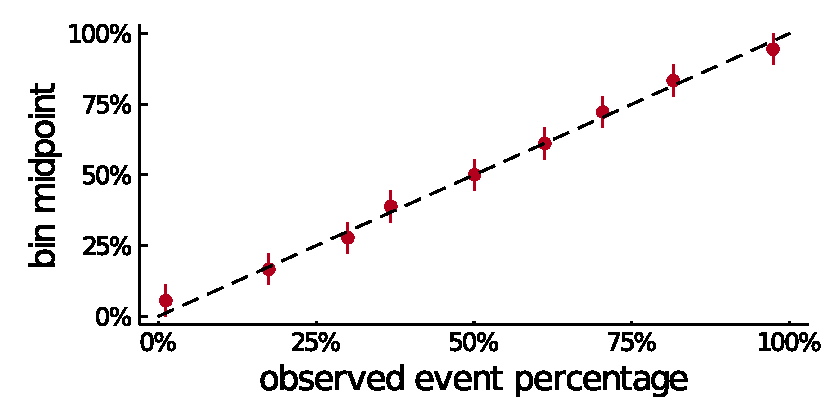
\includegraphics[width=1\linewidth]{plots/phylogeny_calibration.pdf}
  \caption{Calibration plot for the HBV dataset. For a description of all datasets used in this study see section~\ref{sec:results}. Calibration plots for the other datasets are shown in the supplementary.
  All observations are first sorted by increasing estimated probability \(P(y_{ik}=1|\Psi)\) and then grouped into \(n\) bins.
  For each bin, the fraction of observations with \(y_{ik}=1\) (observed event percentage) is compared to the midpoint of each bin (the value in the center between the lowest and highest probability). The error bars show the cutpoints for each bin. If the probabilities are calibrated correctly, each dot is supposed to scatter closely around the diagonal line.}
  \label{fig:phylogeny-calibration}
\end{figure}

The estimated probabilities are then included in the model as additional intercepts:

\begin{equation}
\begin{aligned}
  y_{ik}  & \sim \text{Bernoulli}(\theta_{ik}) \\
  \theta_{ik}  & =  \text{logistic}\Bigl(\beta_{0_{k}} + \gamma~\text{logit}\left(P(y_{ik}=1|\Psi)\right) \\
  &\;\;\;\;\; + \sum_{k=1}^{D}X_{ik}\beta_{\text{HLA}_{jk}}\Bigr)
  \label{eq:phylogeny}
\end{aligned}
\end{equation}

The logit transform is used because is cancels out with the logistic inverse link function. This means that the phylogeny information acts as a baseline in absence of any HLA effects. Note that we also include an additional parameter \(\gamma\), that is constrained to be positive. This helps because the inferred probabilities \(P(y_{ik}=1|\Psi)\) might not necessarily reflect the true underlying phylogenetic signal, for example because the phylogenetic tree does not match the observed data well enough.

A straight-forward extension of our model would be to also account for these sources of uncertainty, for example by using a Bayesian method to estimate a posterior distribution over possible tree topologies. The uncertainty over the tree topology and the underlying parameters of the phylogenetic model would then propagate into uncertainty of the estimated probabilities \(P(y_{ik}=1|\Psi)\). However, in order to not increase the runtime of the model further we  use standard maximum likelihood estimates and then include these in a way that additionally allows for measurement error.

\textit{Binding affinity prediction}

\hl{DaHo: Mein Verständnis von Materials and Methods ist, dass hier die Methoden aufgeführt werden, z.B. die Methoden für die Berechnung von Affinitäten, siehe z.B. https://academic.oup.com/bioinformatics/article/36/21/5159/5874440}
  
    HAMs are expected to lie more frequently in T-cell epitopes, i.e.\ the peptide fragments presented by MHC to T-cell receptors. There are vast experimental binding affinity data available of different peptides and MHC I molecule pairs, and there are well-established computational methods that use these data to extrapolate HLA binding for untested peptides. We show that, by including the outcome of these computational tools as input for a probabilistic model, the prediction of HLA-associated mutations can be improved.

  \textit{Antigen processing prediction}
  
    Similarly, there are also HLA-allele independent effects like antigen processing that influence presentation on MHC I. Second generational tools like MHCFlurry 2.0~\citep{ODonnell2020} use both binding affinity and antigen processing data to improve epitope prediction. For our tool HAMdetector, we use the output of MHCFlurry to benefit from this data in order to predict HLA-associated mutations.

    \subsubsection{Epitope predictions}

There is vast experimental data on epitope binding motifs available, e.g. through the use of mass spectrometry~\citep{Hunt1992}. Epitope prediction software like MHCFlurry~\citep{ODonnell2020} use these data to extrapolate MHC I binding for new, untested peptides.
As HLA-associated mutations are much more likely to lie in epitopes (e.g. because of selection pressure to escape MHC I binding), using epitope prediction software can provide valuable external data for identifying HLA-associated mutations.

For our model, we use MHCFlurry 2.0 for binding prediction, as it does not only predict HLA binding but also antigen processing. For this, we create an input matrix of dimensions \(R\times D\), where R is the number of evaluated replacements and D is the number of observed HLA alleles in the dataset. The elements of this matrix are binary encoded and contain a 1 if that position is either expected to be inside a predicted epitope or related to antigen processing, and 0 otherwise. Given an amino acid sequence, MHCFlurry 2.0 provides a list of possible epitopes (9-13 mers) and HLA allele pairs and calculates a rank based on comparisons with random epitope and HLA pairs. For the binarization we use a rank threshold of 0.2\% (as suggested by MHCFlurry).

We typically try to avoid thresholds whenever possible, but in this case we deemed it to be preferable to including the predicted binding affinities, as we expected the binary values to be more reliable than the predicted numeric values.
Note that the output of these epitope prediction tools may be imprecise or even wrong, but by including it as an input for a probabilistic model, the model is able to learn how much to trust this data if parameterized in a way to allow for measurement error.

We use epitope prediction as information about the expected degree of sparsity, i.e. when knowing a certain position is restricted by a certain HLA allele, we expect that this HLA allele is more likely to be associated with the replacement than the other HLA alleles.
This can be reflected by increasing the scale of the local shrinkage parameters \(\lambda_{jk}\):

\begin{equation}
  \begin{aligned}
    \lambda_{jk} &\sim \text{Cauchy}^{+}(0, \text{exp}(Z_{jk}\beta_{\text{epi}})) \\
    \beta_{\text{epi}} &\sim \text{Normal}^{+}(1, 2),
  \end{aligned}
\end{equation}
 
where \(Z_{jk}\) is 1 if HLA allele \(j\) is predicted to restrict the alignment position corresponding to replacement \(k\) or is associated antigen processing and 0 otherwise.
The parameter \(\beta_{\text{epi}}\) governs the increase in scale of the  corresponding local shrinkage parameters. The larger the estimated values of \(\beta_{\text{epi}}\) are, the more likely it is to see non-zero regression coefficients for these HLA alleles.

\subsection{Sparsity-inducing priors}
  
  Recent advantages in Bayesian inference include so-called sparsity-promoting priors~\citep{Piironen2017}. Sparsity-promoting priors convey the a priori expectation that most coefficients in a regression model are close to 0. This assumption also applies to HLA-associated mutations, because the number of epitopes that are restricted by a given HLA allele is typically small compared to the number of all possible epitopes. If no epitope spanning a given alignment position is presented on the MHC I molecule, any association between a replacement and the respective HLA allele  is likely to be due to random variation alone (or HLA linkage disequilibrium).
  
  It has been shown \hl{DaHo: where?} that using a sparsity-promoting prior when non-zero coefficients are sparse can drastically improve predictive performance, because the model is better able to differentiate between signal and noise.

  We show that a simple logistic regression model with a sparsity-promoting prior on the regression coefficients for the HLA alleles alone already performs roughly on-par  with the much more elaborate Phylogenetic Dependency Network approach from Carlson et al. when using the fraction of identified escapes that lie in known HLA epitopes as a benchmark.

In the context of identifying HLA associations we expect most of the HLA coefficients to be very close to 0, as a given alignment position is typically only restricted by none or few HLA alleles.
This is important prior knowledge that should be incorporated in the model.

For Bayesian models, there are a variety of different sparsity-promoting priors with slightly different properties. They share the common structure of placing most probability mass very close to 0, with large to tails to accommodate the non-zero coefficients.
For our model, we use a so-called horse prior~\citep{Carvalho2010}, which is defined as a scale-mixture of gaussians:

\begin{equation}
  \begin{aligned}
    \beta_{jk} &\sim \text{Normal}(0, \tau^{2}\lambda^{2}_{jk}) \\
    \lambda_{jk} &\sim \text{Cauchy}^{+}(0, 1) \\
    \tau &\sim \text{Cauchy}^{+}(0, \tau_{0})
  \end{aligned}
\end{equation},
where \(\beta_{jk}\) are the regression coefficients, \(\tau\) is the so-called global shrinkage parameter, \(\lambda_{jk}\) are the so-called local shrinkage parameters and \(\text{Cauchy}^{+}\) is the positively constrained Cauchy distribution.

Intuitively speaking, the global shrinkage parameter \(\tau\) is typically very small and shrinks most of the regression coefficients to 0, whereas the local shrinkage parameters can occasionally be very large to allow some coefficients to escape that shrinkage.

A useful addition to the horseshoe prior is given in \citet{Piironen2017}, which describes a way to choose the parameter governing the overall degree of sparsity \(\tau_{0}\) based on the expected number of non-zero coefficients. 

For our HLA model, we utilize an extension to the horseshoe prior called the regularized horseshoe prior~\citep{Piironen2017}, which also provides some regularization for the non-zero coefficients. This is particularly useful for logistic regression models, as some shrinkage helps to deal with issues of separability and collinearity that commonly occur when fitting logistic regression models.

\subsection{Full model specification}

The full specification of the model is given by:

\begin{equation}
  \label{eq:full}
  \begin{aligned}
   y_{ik} &\sim \text{Bernoulli}(\theta_{ik}) &\\
   \theta_{ik} &=
        \text{logit}^{-1}(\beta_{0_{k}} + \gamma_{k}\text{logit}(P(y_{ik}=1|\Psi)) & \\
        \hspace{-6cm} &~~~~ +\sum_{k=1}^{D}X_{ij}\beta_{\text{HLA}_{jk}}) & \\
    \beta_{0_{k}} &\sim \text{Normal}(0, 100^2) & \text{(*)}\\
   \gamma_{k} &\sim \text{Normal}(\mu_{\text{phy}}, \sigma_{\text{phy}}^2) & \\
    \mu_{\text{phy}} &\sim \text{Normal}(1, 1) & \text{(*)} \\
   \sigma_{\text{phy}} &\sim \text{Normal}^{+}(0, 0.5) & \text{(*)} \\
   \beta_{\text{HLA}_{jk}} &\sim \text{Normal}(0, \tau_{k}^{2}\tilde{\lambda}^{2}_{jk}) & \\
   \tilde{\lambda}^{2}_{jk} &= \frac{c_{k}^{2}\lambda_{jk}^{2}}{c_{k}^{2} + \tau_{k}^{2}\lambda_{jk}^{2}} & \\
    c_{k}^2 &\sim \text{Inv-Gamma}(3.5, 3.5) & \text{(*)} \\
   \lambda_{jk} &\sim \text{Cauchy}^{+}(0, \sigma_{j}^2\text{exp}(Z_{jk}\beta_{\text{epi}})) & \\
   \tau_{k} &\sim \text{Cauchy}^{+}(0, \tau_{0k}) & \text{(*)} \\
   \tau_{0k} &= \frac{10}{D-10}\frac{2}{\sqrt{N}} & \\
  \end{aligned}
\end{equation}

The full model specification includes some aspects that were not covered in the previous sections. In particular, the parameters \(\gamma_{k}\) are modelled hierarchically, which allows information to be partially pooled across replacements. However, the model would also work reasonably well with just a single global parameter \(\gamma\). All other additions (\(\tilde{\lambda}_{jk}^{2}\) and \(\tau_{0k}\)) are explained in detail in \citep{Piironen2017}. Briefly, the addition of  \(\tilde{\lambda}_{jk}^{2}\) allows some regularization for the non-zero coefficients and the parameterization of \(\tau_{0k}\) allows to place a prior on the expected number of non-zero coefficients.

\subsubsection{Prior justification}

Prior distributions are labeled with an asterisk in equation~\ref{eq:full}. They are meant to be weakly informative, which means that the goal is to provide some modest amount of shrinkage while still allowing for large absolute values given enough support by the observed data. One exception to this are the intercepts \(\beta_{0_k}\), which are essentially flat because they are well identified by the data alone.

The hierarchical mean and standard deviation of the phylogeny coefficients \(\gamma_{k}\) are chosen to place most probability mass at values of \(\gamma_{k}\) of around 1. In the absence of any HLA effects, a parameter value of 1 would mean that the estimate for the probability of observing replacement \(k\) is identical to the probability based on the phylogenetic model. Intuitively speaking, We therefore treat the phylogeny as a baseline and any observations that cannot be attributed to phylogeny are attributed to the HLA alleles or noise.

The prior on \(c_{k}^{2}\) implies a Student-t prior with 7 degrees of freedom and a scale of 1 on the non-zero HLA regression coefficients \(\beta_{\text{HLA}_{jk}}\). A Student-t prior with these parameters is a reasonable default choice for logistic regression models. The theoretical justification behind this regularized variant of the horseshoe prior is explained in detail in \citet{Piironen2017}.

The value of \(\tau_{0k}\) is chosen to imply 10 effective non-zero HLA regression coefficients per replacement. The rationale behind this parameterization is again outlined in \citet{Piironen2017}. The value of 10 is approximately based on available HIV epitope maps. Please note that this is only an approximate statement about the general magnitude, i.e. we would expect maybe a couple of HLA alleles to be associated with a single replacement, not much more.
The model is also parameterized in a way that assumes an equal degree of sparsity across all alignment positions a priori. We also tried to model \(\tau_k\) hierarchically, but observed sampling issues due to the resulting unfavorable geometry of the posterior.


\subsection{Model implementation}
All models were implemented in Stan~\citep{Stan2021}. The Stan code is available online in two versions: One optimized for readability and one optimized for speed by utilizing Stan's multithreading and GPU capabilities.
A Julia~\citep{Bezanson2017} package is available \hl{DaHo: at ...} to run the model on custom data. Due to restrictions of dependencies (MHCFlurry and RAxML-ng), HAMdetector is only available on Linux. %We additionally provide Docker images to easily run the model on any operating system in a containerized environment, assuming Docker is installed. 


  \subsection{Model diagnostics}

  \subsubsection{Posterior predictive checks}

  Additionally, Bayesian statistics provides an accessible way to test models: By comparing data generated under the model's assumptions to the actually observed data, it is possible to identify important aspects of the dataset that the models fails to capture and subsequently improve the model until it is consistent with the observed data~\cite{Gabry2019}.

  Here, we use these so-called posterior predictive checks to compare the calibration of the predicted probabilities of observing the replacement to the actual observed data. 

  \subsubsection{Convergence diagnostics}

  We use Stan (version 2.23)~\cite{Stan2021} to specify and fit our Bayesian models.
  Stan provides an implementation of a dynamic Hamilitonian Monte Carlo sampler, which is a powerful technique to approximate expectations with respect to the posterior distribution~\cite{Betancourt2017}. One advantage of using such methods is that they provide sensitive diagnostics to identify a wide range of possible sampling issues.
  We use the split-\(\hat{R}\) convergence diagnostic~\cite{Gelman1992} to identify convergence issues. We require a value of \(\hat{R}\) below 1.01 for all model parameters. Additionally, we require that the effective sample size \(N_{\text{eff}}\) is above 500 for all model parameters and that sampling occurs without any divergent transitions. A detailed explanation of these quantities is provided in the Stan reference manual.

  \subsubsection{Leave-one-out cross-validation}

  In addition to testing our model on real-world data, we also performed leave-one-out cross-validation to examine the relative importance of the additions of epitope prediction, sparsity and phylogeny with respect to predictive performance.
  For this, we create several variations of the model that are all special cases of the full HAMdetector model.
  By comparing the model performance of these variations, we can gain insight on the relative importance of each aspect of the model.
  
  Leave-one-out cross-validation has historically been challenging to apply for Bayesian models, because fitting a model once for each left out data-point is often infeasible because of computational constrains.
  Recently, Pareto-smoothed importance sampling has gained popularity to perform approximate leave-one-out cross-validation for Bayesian models. This method  approximates the leave-one-out posterior by re-weighting existing draws from the posterior distribution and has the advantage of requiring to fit the model only once. Additionally, the method provides good diagnostics to identify cases where the approximation is unreliable~\cite{Vehtari2016}.

  Several utility (or cost) functions are used in practice to compare the predictive performance of models. For frequentist approaches, classification accuracy or receiver operator characteristic curves (ROC curves) are most common.
  For Bayesian models, expected log-predictive density (elpd) is used most frequently. 

  elpd is defined as \(\sum_{i=1}^{n}\text{log}(\int p(y_i|\theta)p(\theta|y_{i-1})d\theta))\), i.e. the average log predictive density of the observed data points based on the leave-one-out posterior distributions.
  This has the advantage over other performance measures like classification accuracy, that it not only takes the location of the predictive distribution into account (i.e. the number of correct predictions), but also the width (i.e. how confident the model is in its predictions).
  elpd cannot be computed for frequentist models because the parameters of the model are viewed as fixed values.

  \subsection{Data and data preparation}
 \hl{DaHo: das Material in Materials and Methods sind die Daten; die sollten hier kurz beschrieben werden, möglichst mit Referenzen}

The model was fit with several data sets:

\begin{itemize}
  \item A large HIV dataset consisting of 1383 sequences, that were kindly provided by Zabrina Brumme and collaborators and were also used in the Phylogenetic Dependency Network study~\citep{Carlson2008}.
  \item A set of 351 HIV sequences mostly spanning the Pol gene from the Arevir database~\citep{Roomp2006}.
  \item A set of 544 Hepatitis-B-Virus sequences that were kindly provided by Jörg Timm.
  \item A set of 104 Hepatitis-D-Virus sequences that were kindly provided by Michael Roggendorf. \hl{DaHo: bitte von Hadi geeignetes Zitat erfragen}
  \item A set of 41 HIV sequences that were kindly provided by Rongge Yang. 
\end{itemize}

\hl{DaHo: zu jedem Datensatz die Proteine nennen}

For all sequences, we applied the following data preparation steps:

\begin{enumerate}
  \item For each dataset, the sequences were split into subsequences, either by protein or gene.
  \item If not already present in this format, sequences were translated into their amino acid representation.
  \item RAxML-NG~\citep{Kozlov2019} version 1.0.0 was used to generate a maximum likelihood phylogenetic tree for each gene/protein using the \texttt{--model GTR+G+I} option with all other parameters set to default values. If available, we used RNA or DNA sequences for this step, rather than protein sequences.
\end{enumerate}

\end{methods}

\section{Results} \label{sec:results}

In order to evaluate each building block of HAMdetector, we applied 4 different Bayesian models to each dataset, each of which includes the previous model as a special case:
A standard logistic regression model, a logistic regression model with horseshoe prior, a model additionally including phylogeny and the full model with horseshoe prior, phylogeny and epitope prediction.
As a comparison to existing methods, we also applied Fisher's exact test and the Phylogenetic Dependency Network.

\subsection*{Convergence diagnostics}

 All model fits showed no signs of inference issues. In total, samples were drawn from 4 different chains with 1000 iterations each. The effective sample size exceeded 500 for all model parameters, \(\hat{R}\) convergence diagnostic values were below 1.01 in all cases. \hl{DaHo: citation Gelman + Rubin original paper or later versions if improved $\hat{R}$ have been used}

\subsection*{Posterior predictive checks}

Figure~\ref{fig:calibration} compares the calibration of the posterior predictive probability of observing the replacement to the actual observed data for the Core protein of the HBV dataset. Plots for the other models and datasets are shown in the supplementary.

The plots are similar to the one showed in figure~\ref{fig:phylogeny-calibration}, however, they do not evaluate the probabilities based on the phylogenetic model alone, but instead show the calibration of the posterior predictive probabilities based on the full model.

\begin{figure}[!ht]
  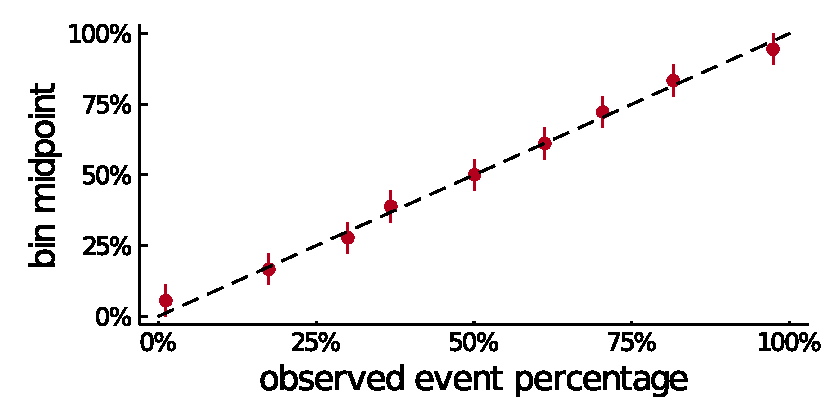
\includegraphics[width=1\linewidth]{plots/phylogeny_calibration.pdf}
  \caption{Calibration plot for the HBV dataset. Calibration plots for the other datasets are shown in the supplementary.
  All observations are first sorted by increasing estimated probability \(P(y_{ik}=1)\) and then grouped into \(n\) bins.
  For each bin, the fraction of observations with \(y_{ik}=1\) (observed event percentage) is compared to the midpoint of each bin (the value in the center between the lowest and highest probability). The error bars show the cutpoints for each bin. If the probabilities are calibrated correctly, each dot is supposed to scatter closely around the diagonal line.}
  \label{fig:calibration}
\end{figure}

\subsection*{Comparison to a list of known epitopes}

When testing models, we prefer to evaluate them on real-world data whenever possible. 
However, comparing against real-world data is not straight forward when identifying HLA-associated mutations, because if a tool identifies an HLA-associated mutation which is not yet documented, this could be either because it is a false positive, or a yet unknown HLA-associated mutation that has not been documented before. 
Also, viewing every non-identified HLA-associated mutation that is listed in the literature as a false negative is not correct either, because documented escape mutations do not necessarily have to show in each sequence alignment.
A third issue when comparing models is that HLA-associated mutations are not necessarily binary, so the true positive / false negative framework does not work as well.

To circumvent these issues and still compare against real-world data, we chose the following strategy:
For each model, all evaluated replacements are ranked by decreasing confidence of being an HLA associated mutation. That is, for Bayesian models we calculate the probability of the corresponding regression coefficient exceeding zero \(P(\beta_{HLA} > 0)\), for Fisher's exact test we sort HLA allele - replacement pairs by increasing p-values and for the Phylogenetic Dependency Network, we rank the associations by increasing q-values.
Then, a list of known epitopes is used to create a plot of the cumulative number of replacements inside the boundary of a known epitope vs. the corresponding rank. The underlying assumption for this kind of model check is that we expect to see an enrichment of replacements that lie inside the region of known epitopes and that this enrichment is stronger for better performing models.

\begin{figure}[ht!]
  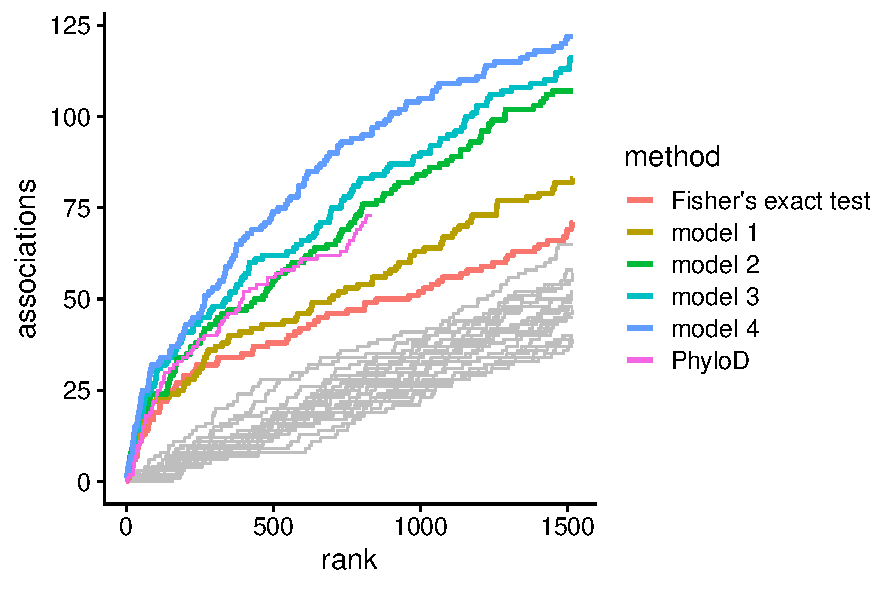
\includegraphics[width=1\linewidth]{plots/comparison.pdf}
  \caption{Number of associations inside the boundary of known epitopes vs. rank. For each model, the pairs of HLA alleles and replacements are sorted by decreasing confidence of being an HLA associated mutation. Then, each replacement is compared to a list of known epitopes and a line of the cumulative number of associations inside known epitopes vs. the current rank is plotted for each model. Better performing models are expected to have an enrichment of associations that are inside of known epitopes. 
  PhyloD: Phylogenetic Dependency Network, Model 1: simple logistic regression model with broad Student-t priors, Model 2: logistic regression model with horseshoe prior, Model 3: logistic regression model with horseshoe prior and phylogeny, Model 4: Full model with epitope prediction. The thin gray lines denote random permutations of the list of HLA allele - replacement pairs and act as a baseline.}
  \label{fig:comparison}
\end{figure}

Figure~\ref{fig:comparison} shows a comparison of different models on the HBe protein of the HBV dataset. Plots for all other datasets are shown in the supplementary, but show identical patterns.

All models show a strong enrichment of HLA-associated mutations compared to a randomly permuted list of HLA allele - replacement pairs (gray lines). Fisher's exact test performs about as well as the simple logistic regression model, as from a statistical perspective, they are both similar.
The horseshoe prior alone is a drastic improvement over Fisher's exact test and the logistic regression model with non-sparsifying priors, even though it does not include any external information. The benefit comes from including the assumption that most regression coefficients are expected to be very close to 0.
The logistic regression model with horseshoe prior works roughly as well as the Phylogenetic Dependency Network, which includes much more information.
Note that the line for the Phylogenetic Dependency Network is shorter because it only outputs associations with a q-value lower than 0.2 by default.

The remaining models are ranked in order of the number of additional features they include. Additionally including phylogeny is a small improvement over the model with the horseshoe prior, while adding epitope prediction provides another strong improvement.

Note that this model only uses epitope \textit{prediction} software and does not use any information of experimentally confirmed epitopes. These are here only used for model evaluation.

Figure~\ref{fig:horseshoe-comparison} shows a comparison of marginal posteriors for regression coefficients with and without horseshoe prior.

Supplying information about the expected degree of sparsity with the horseshoe prior is a considerable improvement over a standard logistic regression model  (section~\ref{sec:results}).

\begin{figure}
  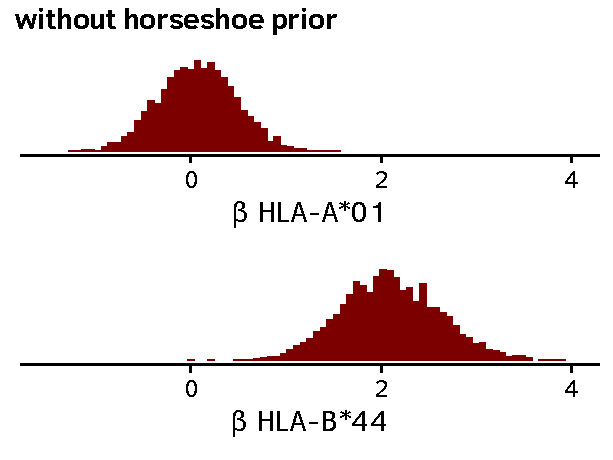
\includegraphics[width=1\linewidth]{plots/without_horseshoe.pdf}
  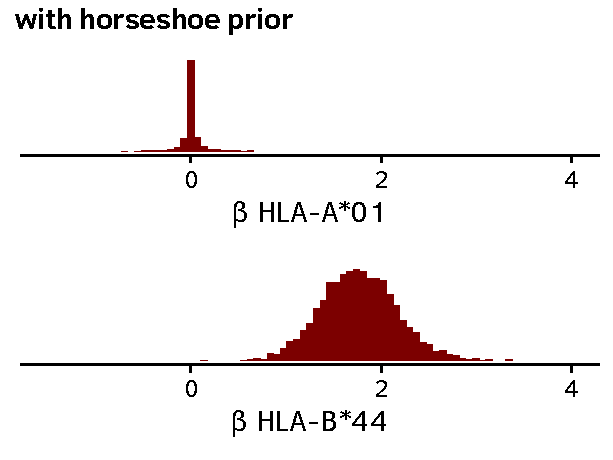
\includegraphics[width=1\linewidth]{plots/with_horseshoe.pdf}
  \caption{Marginal posterior distributions of a subset of regression coefficients for replacement 11D of the HIV integrase, based on the Arevir dataset. The graphic shows regression coefficients for two HLA alleles: For HLA-A*01, the data does not show evidence of an association with replacement 11D, whereas for HLA-B*44, the data is consistent with a strong association. The horseshoe prior has the effect of shrinking regression coefficients with weak evidence of an association with the replacement strongly towards 0, while leaving the coefficients that are far away from 0 mostly unshrunk. Shrinking the irrelevant regression coefficients to 0 has the advantage of reducing the standard error for the remaining coefficients, which can be observed by the much smaller width of the histogram of HLA-B*44 in the model with horseshoe prior.}
  \label{fig:horseshoe-comparison}
\end{figure}


\subsection{Leave-one-out cross-validation}

Table \ref{loo} shows a comparison of models with increasing complexity run on the HBe protein in the HDV dataset.

\begin{table}[h!]
  \renewcommand{\arraystretch}{1.3}
  \centering
  \caption{Differences in elpd for models with increasing model complexity (HBe protein of the HBV dataset).
  The numbers in column \(\text{elpd}_\text{diff}\) show increases in elpd compared to the previous model (higher is better), e.g. the difference in elpd of the model with horseshoe prior is 949.8 compared to the baseline model, and the difference in elpd for the model with phylogeny and horseshoe prior is 4440.9 compared to the model just with the horseshoe prior. All differences in elpd are larger than several times the estimated standard error (column \(\text{se}_\text{diff}\)), indicating that models which account for more information are expected to have a better predictive performance.}
  \vspace{0.5cm}
  \begin{tabular}{l|r|rll}
  \multicolumn{1}{l|}{} & \multicolumn{1}{c|}{\(\text{elpd}_\text{diff}\)} & \multicolumn{1}{c}{\(\text{se}_\text{diff}\)} &  &  \\ \cline{1-3}
  logistic regression (baseline) & 0.0  & 0.0 &  &  \\
  + horseshoe prior     & 949.8  & 65.2 &  &  \\
  + phylogeny & 4440.9 & 94.4 &  &  \\
  + epitope prediction & 63.1   & 18.9 &  & 
  \end{tabular}
  \label{loo}
\end{table}

Predictive accuracy increases as the models include more and more information.
Note that the model with horseshoe prior alone already has a much higher elpd than the standard logistic regression model, even though it does not use any additional external data. This is because including the sparsity assumption allows the model to better separate signal from noise and the uncertainty of the close-to-zero coefficients does not propagate into uncertainty of the estimated y.

Including phylogeny further improves model performance, as the assumption of independent and identically distributed data does not hold for sequence data that share a common phylogenetic history.

Inclusion of epitope prediction does not improve elpd as much as inclusion of phylogeny and the sparsity assumption. This is because while addition of sparsity and phylogeny has an effect on all replacements and samples, epitope prediction only influences those replacements which are restricted by a given HLA allele and only those samples which are annotated with the allele. However, inclusion of epitope prediction is highly useful for determining which HLA alleles are associated with the occurrence of a replacement, as shown in the previous section.

\subsection{Generalization}

\hl{DaHo: Es gibt fast keinen Text in dieser subsection}

The models were applied on sequence data from a variety of different viruses and show a considerable improvement over currently applied methods that are consistent across datasets.
These results are not due to overfitting, because leave-one-out cross-validation approximates the model performance on unseen data.

\subsection{Example Hepatitis Delta Virus}

We had the opportunity to test our model against a set of associations identified by Fisher's exact test where some of them turned out to be false positives~\cite{Karimzadeh2019}. This data is rare because negative results are usually not published in the literature, but provide a useful way to access model performance.
A comparison with a preliminary version of HAMdetector was published recently. Here we provide a comparison with results from Fisher's exact test~\cite{Budeus2016} and the mature version of HAMdetector used in this work.

Fisher's exact test and HAMdetector were applied to the same data (table~\ref{tab:false-positives}).
The posterior probabilities given by HAMdetector denote the probability that the corresponding regression coefficient is positive. Associations with strong support in our model have a posterior probability close to 1, associations with no support a probability close to 0.5 (corresponding to a regression coefficient centered around 0).

The results show low posterior probabilities for most of the false-positives and high posterior probabilities for most replacements that could be experimentally validated in IFN-\(\gamma\) production assays.
One important exception is P89T~-~HLA-B*37, which was experimentally validated but does not have strong support in our model.

\begin{table}[h!]
  \caption{List of HLA associated mutations that were identified using Fisher's exact test (FET). Experimental validation showed that 9 out of 15 replacements could not be experimentally validated (column “confirmed“). The data were re-analyzed using HAMdetector. Except for P89T, all validated replacements have high posterior probabilities, while the replacements that could not be experimentally validated have lower evidence of being HLA associated. Note that all replacement - HLA allele pairs had low p-values using Fisher's exact test.}
  \vspace{0.5cm}
  \begin{tabular}{c|c|c|c|c}
  replacement & allele  & p-value (FET) & post.~prob. & confirmed \\
  \hline
  S170N       & B*15 & \(3\cdot10^{-8}\)      & 0.99                                & +                        \\
  D101E       & B*37 & 0.0002                        & 0.96                                & +                        \\
  R105K       & B*27 & 0.0011                        & 0.93                                & +                        \\
  R139K       & B*41 & 0.0034                        & 0.91                                & +                        \\
  E47D        & B*18 & 0.0027                        & 0.89                                & +                        \\
  D33E        & B*13 & 0.0001                        & 0.86                                & -                        \\
  T134A       & A*68 & 0.0045                        & 0.82                                & -                        \\
  K43R        & B*13 & 0.0021                        & 0.77                                & -                        \\
  D47E        & A*30 & 0.0010                        & 0.76                                & -                        \\
  K113R       & B*13 & 0.0043                        & 0.76                                & -                        \\
  P89T        & B*37 & 0.0011                        & 0.75                                & +                        \\
  A107T       & B*14 & 0.0028                        & 0.70                                & -                        \\
  P49L        & A*30 & 0.0031                        & 0.63                                & -                        \\
  Q100L       & B*13 & 0.0018                        & 0.61                                & -                        \\
  D96E        & B*13 & 0.0035                        & 0.50                                & -                       
  \end{tabular}
  \label{tab:false-positives}
 \end{table}

 \subsection{Individual examples}
In the following we illustrate with ... examples the effects of the inclusion of additional relevant information on the detection of HAMs.
 
 \hl{DaHo: bitte Beispiel mit Linkage Disequilibrium zeigen}

\hl{DaHo: bitte konkretes Bsp mit Auswirkung Phylogenie zeigen}

\section{Discussion}

We have presented HAMdetector, a Bayesian model to identify HLA-associated mutations in a multiple sequence alignment. We propose to use models that include as much information as possible and have shown that including sparsity and epitope prediction software can achieve better performance than existing methods. The logistic regression backbone can be easily extended, which allows the model to also be used in other contexts, for example in identifying associations between sequence data and other features.

If the quality of the prediction is the same for all viruses, as it appears to be in our results, this method can be used to probe the frequency of HLA immune escape across different viruses.

In further research we plan to use HAMdetector to study circulating recombinant forms in HIV. One possible explanation for the occurrence of these recombinant forms is improved fitness by evading several immune epitopes at once.

While our model is an improvement over existing methods, a further addition that we plan to implement is partial pooling across 4-digit HLA alleles. It has recently been appreciated that binding specificities can vary drastically across  HLA alleles from the same allele group. For predicting HLA associated mutations, there has consequently been a shift to use 4-digit resolution data whenever available. 

This is not without downsides however, because overall, binding specificities are more similar for alleles in the same group, and, therefore, treating them as completely separate might unnecessarily fragment the available data.

In Bayesian statistics, it is not required to chose one extreme or the other, With partial pooling, estimates from the same allele group do share some information across each other, but they are also allowed to vary if necessary.
Therefore, implementing partial pooling might be another possibility to further increase the reliability of computational methods to study HLA escape.

%%%%%%%%%%%%%%%%%%%%%%%%%%%%%%%%%%%%%%%%%%%%%%%%%%%%%%%%%%%%%%%%%%%%%%%%%%%%%%%%%%%%%
%
%     please remove the " % " symbol from \centerline{\includegraphics{fig01.eps}}
%     as it may ignore the figures.
%
%%%%%%%%%%%%%%%%%%%%%%%%%%%%%%%%%%%%%%%%%%%%%%%%%%%%%%%%%%%%%%%%%%%%%%%%%%%%%%%%%%%%%%






% \section{Conclusion}



%\section*{Acknowledgements}


\section*{Funding}

This work has been supported by Deutsche Forschungsgemeinschaft (grant HO 1582/10-1).\vspace*{-12pt}

\bibliographystyle{natbib}
%\bibliographystyle{achemnat}
%\bibliographystyle{plainnat}
%\bibliographystyle{abbrv}
%\bibliographystyle{bioinformatics}
%
%\bibliographystyle{plain}
%
\bibliography{references}
\end{document}
